\chapter{Background and Related work}
\label{chap:background}

In this thesis we often operate with such concepts as webpage, HTML, CSS and JavaScript, web element, DOM, XPath, etc. All these terms refer to the field of web development. In this chapter we will discuss the meaning of this concepts as well as main related works in this field.\\

We will start from the webpage and its main components. Then we will explain in details the algorithm of web page rendering, so called the critical rendering path. After we will talk about Web extraction and list the most popular techniques. In the last section we will discuss related main works in the field of Web Extraction, specially those ones which related to the extraction of events and other specific structured information.\\

\section{Web page}
\textit{A Webpage} is primarily text document formatted and annotated with Hypertext Markup Language (HTML). A website is a collection of related webpages together with corresponding media files. To view a rendered webpage, we need to make use of a web browser, which provides communication between the user, webpage resources and web server where the corresponding website is hosted. To get the information needed for a displaying a webpage the browser retrieves the data from a web server by sending HTTP requests. We won't discuss the process of requesting, rather we will explain the intermediate steps between the stage when the browser retrieved the information from the server and displays it to the user.\\ 

There are two main types of the website and therefore the pages - \textit{static} and \textit{dynamic}. A static webpage is usually written in a plain HTML, whereas dynamic page is using a server-side scripts for the content generation. The main points which make the differences between them are scalability, simplicity to update the content and the price. With dynamic websites it is easy to create a big number of similar pages and dynamically update the content based on user actions. Dynamic pages is taking it's content from a database, whereas the static pages already has some content which can't be updated easily. But at the same time with dynamic website it is more complicated to change the design, because the pages are essentially a template into which content is poured to. The design of static pages is more flexible and can be changed manually. As for the price, static website is relatively cheap and easy to make comparing to dynamic websites.\\ 

Anyways, after the browser retrieved the information from the server, for both dynamic and static webpages the browser has the same types of information in order to display the webpage. Only in static case the browser retrieved original files (HTML, CSS, JavaScript, etc)  with the predefined content, and in the dynamic case the web server generated these files and took the data from a database.\\

A webpage as a set of available information contains a lot of different pieces:

\begin{itemize}
    \item The textual information which we see
    \item HTML code with the content, hyperlinks, buttons and other components which the user can interact with.
    \item Static media files, i.e. images, icons, video files, animated GIF, SVG, textual documents and other attached files.
    \item Dynamic media as Flash, Java applets.
    \item Semantic meta-information about the content of the page.
    \item JavaScript scripts which add interactivity and additional functionality.
    \item Cascading Style Sheets (CSS) files which define how to rendered the webpage and set such properties as a font size, distances between blocks, colors, etc. There are more than five hundreds different CSS properties there.
\end{itemize}

\subsection{HTML, CSS and JavaScript}
The triad of the most important Web technologies are HTML to specify the content of web pages, CSS to specify the presentation of web pages, and JavaScript to specify the behaviour of web pages.[source Flanagan, David. JavaScript - The definitive guide (6 ed.). p. 1.]. Let's briefly discuss how these three major components looks like and show small examples.\\
[source https://www.w3schools.com]

\noindent\textbf{Hypertext Markup Language (HTML)} - is the standard markup language for creating web pages and web applications. HTML document has the structure of a tree and contains the configuration of the page, its textual content and links to all associated media files. HTML file is parsed by a browser into Document Object Model and we will consider this process in details in the next section. The building blocks of an HTML is an HTML tags which after the parsing transformed to an HTML elements. Here is an example of the simple HTML document: \\

\begin{lstlisting}[language=html]
<!DOCTYPE html>
<html>
<title>HTML Tutorial</title>
<body>

<h1>This is a heading</h1>
<p>This is a paragraph.</p>

</body>
</html>
\end{lstlisting}

It is possible to incorporate both CSS and JavaScript into the HTML but in a modern web development these three thing are usually separated into different files. It allows to maintain and change the content, the visualization and the interactivity features independently.\\

\noindent\textbf{Cascading Style Sheets (CSS)} is a style sheet language used for describing the presentation of a document written in a markup language [source: "CSS developer guide". Mozilla Developer Network. Retrieved 2015-09-24.]. CSS is primarily designed to enable the separation of content and presentation of a webpage, including layout, colors, and fonts. Such separation improves content accessibility and allows easily change the visual presentation of the page. CSS also allows to control how the page will display on a different screens and devices. There are more than five hundreds available CSS properties which can be specified. Both the CSS and HTML specifications are maintained by the World Wide Web Consortium (W3C). Web browser parses CSS files and creates CSSOM tree which is very conceptually similar to DOM. Here is an example of the simple CSS document: \\

\begin{lstlisting}[language=css]
body {
    background-color: lightblue;
}

h1 {
    color: white;
    text-align: center;
}

p {
    font-family: verdana;
    font-size: 20px;
}
\end{lstlisting}\\

\noindent\textbf{JavaScript (JS)} is a powerful multi-paradigm language, supporting object-oriented, imperative, and functional programming styles [link to Wiki]. 95\% of 10 million most popular web pages use JS, and all modern web browsers support it without the need for plug-ins [https://w3techs.com/technologies/details/cp-javascript/all/all]. Scripts are embedded in or included to HTML pages and interact with the DOM and CCSOM. JS can interact and modify both DOM and CCSOM and it adds interactivity to originaly static webpages. There are come examples of the JS effects:

\begin{itemize}
    \item It allows to load data from the server without needs to reload the page (AJAX technology).
    \item It adds animation, interactivity and media content.
    \item It can track the user behavior on the website and collect the information for the web analytic, ad tracking, and penalization purposes.
\end{itemize}

\begin{lstlisting}[language=JavaScript]
var canvas = document.createElement('canvas');
canvas.width = 100;
canvas.height = 100;

var image = new Image();
image.width = 120;
image.height = 150;
image.onload = window.setInterval(function() {
    rotation();
}, 1000/60);
\end{lstlisting}\\

\subsection{XPath}

\section{How does the browser render the page}

Every time the browser retrieves the information from the web server, it makes the series of important actions in order to display the initial page to the user. This series of steps is named \textit{the critical rendering path}. For a web developers it is very important to understand these steps because optimized websites are easy to use and have a higher rank in search engines. Optimized in this case means that the browser is able to load and render the page quickly and the internal structure of the code is clear.\\

[source: https://developers.google.com/web/fundamentals/performance/critical-rendering-path/adding-interactivity-with-javascript]
[source: https://varvy.com/pagespeed/critical-render-path.html]
The algorithm of how does the browser render the page as follows:

\begin{enumerate}
    \item The browser retrieves the HTML, read it and see that there are CSS and JavaScripts files for this HTML needed.
    \item The browser decides if it's possible to render the page and if yes it loads all necessary resources including CSS, JavaScript and media files.
    \item The browser parses the HTML code and builds the \textit{Document Object Model} (DOM) tree. The DOM contains the objects which define the structure and the content of the page.
    \item The browser parses the CSS files and builds the CSSOM tree. It is very much like DOM for HTML. The CSSOM contains the objects which define the style of all elements in DOM.
    \item JavaScript can modify existing DOM and CSSOM, change any elements of both trees.
    \item The DOM and CSSOM trees are combined to form \textit{the Render tree}. Render tree doesn't include the hidden nodes as script, meta tags, an so on. Also some nodes are hidden because it was reflected in the CSS files (explicit property "display: none"). Render tree contains only the nodes which required to render the page.
    \item The browser is building the layout and computes the exact position and size of each object.
    \item The paint stage is when the browser takes the render tree and renders (meaning draws) the pixels to the screen of the user. 
\end{enumerate}

On the picture \nameref{fig:domcsstree} you can see how the DOM, CSSOM amd Render Tree look like on the \nth{6} step.\\

\begin{figure}[h]
\begin{center}
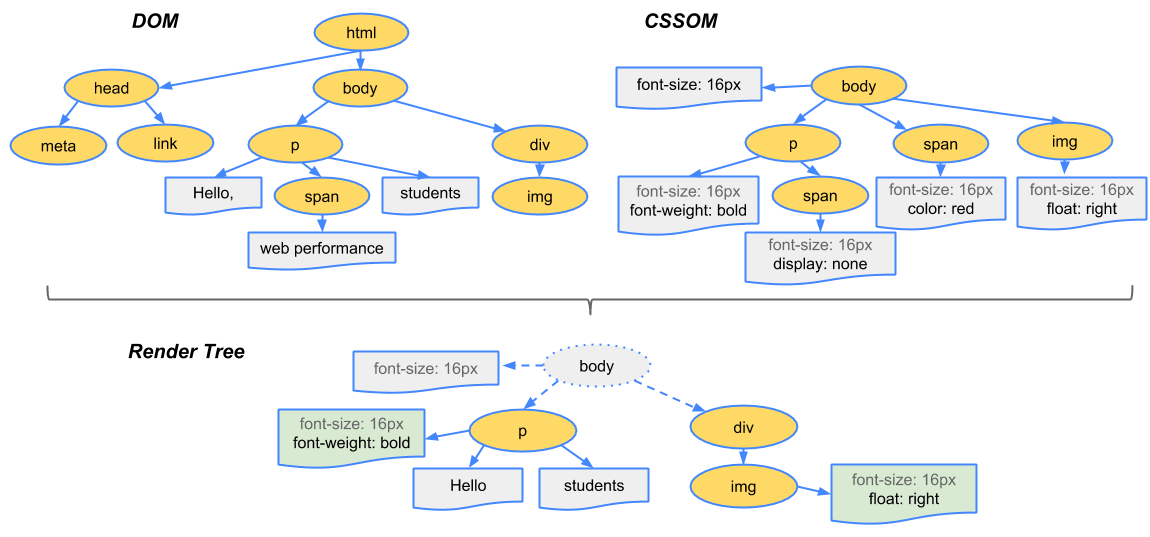
\includegraphics[width=1.0\textwidth]{figures02/render-tree-construction}
\caption{The DOM and CSSOM trees are combined to form the Render tree}
\label{fig:domcsstree}
\end{center}
\end{figure}

The popularity of the website in search engines depends upon several factors: the website has relevant and interesting content, , from developer point of view the website is optimized and has clear internal structure, the website is active and 



\section{Web extraction}

The data in the Internet is very massive and heterogeneous. Every website is following it's own design and structure, presenting the same information in a different way for the specific audience of the website. World Wide Web Consortium (W3C) is an international standard organization. tries to get all the players on the Web implement the same set of core principles and components, use the same technologies and standards. 


\subsection{Web extraction methods}
\subsubsection{Wrappers}
\subsubsection{Adaptive information extraction}
\subsection{Other related techniques}
\subsubsection{Region extraction}
\subsubsection{Visual segmentation}
\subsection{Recall and Precision}
\subsection{Web extraction as a service}
\section{Semantic web}
\subsection{Microformats, RDF}
\subsection{Semantic web pervasiveness}
\section{Related works}


